\documentclass[aspectratio=169,11pt]{beamer}

\usetheme{Madrid}
\usefonttheme{professionalfonts}
\setbeamertemplate{navigation symbols}{}
\setbeamertemplate{footline}[frame number]

\usepackage[T1]{fontenc}
\usepackage{lmodern}
\usepackage{graphicx}
\usepackage{booktabs}
\usepackage{tabularx}
\usepackage{tikz}
\usetikzlibrary{positioning}
\usepackage{xcolor}

\definecolor{DeepBlue}{HTML}{102A43}
\definecolor{Steel}{HTML}{486581}
\definecolor{SoftBlue}{HTML}{E3F2FD}
\definecolor{SoftGreen}{HTML}{E8F5E9}
\definecolor{SoftAmber}{HTML}{FFF8E1}
\definecolor{SoftPurple}{HTML}{F3E5F5}
\definecolor{SoftCyan}{HTML}{E0F7FA}
\definecolor{SoftRose}{HTML}{FCE4EC}
\definecolor{Accent}{HTML}{1976D2}

\setbeamercolor{title}{fg=DeepBlue}
\setbeamercolor{frametitle}{fg=DeepBlue,bg=SoftBlue}
\setbeamercolor{normal text}{fg=DeepBlue}
\setbeamercolor{block title}{fg=white,bg=Accent}
\setbeamercolor{block body}{fg=DeepBlue,bg=SoftBlue}
\setbeamercolor{alerted text}{fg=Accent}

\newcommand{\component}[3]{%
  \begin{block}{#1}
    \textbf{What it does:} #2

    \vspace{0.35em}
    \textbf{Why we used it:} #3
  \end{block}
}

\title[Distributed Web Crawler]{Dockerized Distributed Web Crawler}
\subtitle{Polite Crawling, Shared Storage, Streaming Indexing, and Ranked Search}
\author[Vaibhav, Sayam, Aaditya]{Vaibhav Gupta \and Sayam Agarwal \and Aaditya}
\institute{Project Evaluation Presentation}
\date{\today}

\begin{document}

\begin{frame}
  \titlepage
\end{frame}

\begin{frame}{What We Built}
  \small
  \begin{block}{Project goal}
    Build a distributed web crawler that can run from Docker, crawl pages through multiple worker containers, store crawled data safely, update the search index continuously, and return ranked search results through an API.
  \end{block}

  \begin{columns}[T,totalwidth=\textwidth]
    \begin{column}{0.48\textwidth}
      \begin{block}{Crawler side}
        \begin{itemize}
          \item Redis manages URL scheduling and worker coordination.
          \item Crawler workers fetch pages independently.
          \item Robots.txt and per-domain politeness protect target sites.
          \item MinIO stores raw HTML outside MongoDB.
        \end{itemize}
      \end{block}
    \end{column}
    \begin{column}{0.48\textwidth}
      \begin{block}{Search side}
        \begin{itemize}
          \item MongoDB stores metadata, clean text, graph state, and indexes.
          \item Streaming workers update search data after crawls.
          \item PageRank maintains page authority scores.
          \item FastAPI combines relevance and authority for results.
        \end{itemize}
      \end{block}
    \end{column}
  \end{columns}
\end{frame}

\begin{frame}{End-to-End Flow}
  \centering
  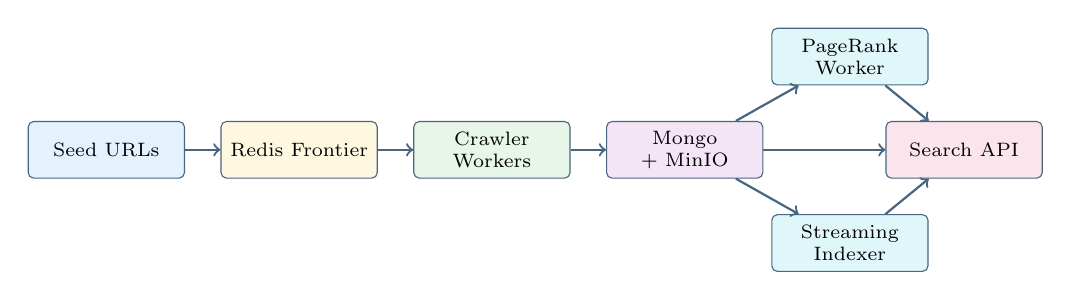
\begin{tikzpicture}[
      node distance=0.45cm,
      every node/.style={font=\scriptsize},
      box/.style={draw=Steel, rounded corners=2pt, minimum height=0.72cm, align=center, text width=1.75cm},
      arrow/.style={->, thick, draw=Steel}
    ]
    \node[box, fill=SoftBlue] (seed) {Seed URLs};
    \node[box, fill=SoftAmber, right=of seed] (redis) {Redis Frontier};
    \node[box, fill=SoftGreen, right=of redis] (worker) {Crawler Workers};
    \node[box, fill=SoftPurple, right=of worker] (storage) {Mongo + MinIO};
    \node[box, fill=SoftCyan, below right=0.45cm and 0.1cm of storage] (index) {Streaming Indexer};
    \node[box, fill=SoftCyan, above right=0.45cm and 0.1cm of storage] (pr) {PageRank Worker};
    \node[box, fill=SoftRose, right=1.55cm of storage] (api) {Search API};

    \draw[arrow] (seed) -- (redis);
    \draw[arrow] (redis) -- (worker);
    \draw[arrow] (worker) -- (storage);
    \draw[arrow] (storage) -- (index);
    \draw[arrow] (storage) -- (pr);
    \draw[arrow] (index) -- (api);
    \draw[arrow] (pr) -- (api);
    \draw[arrow] (storage) -- (api);
  \end{tikzpicture}

  \vspace{0.8em}
  \begin{block}{Flow summary}
    Seed URLs enter Redis. Workers fetch and parse pages. MongoDB commits page data and outbox events atomically. Streaming consumers update search and authority state. FastAPI serves ranked results.
  \end{block}
\end{frame}

\begin{frame}{System Architecture}
  \centering
  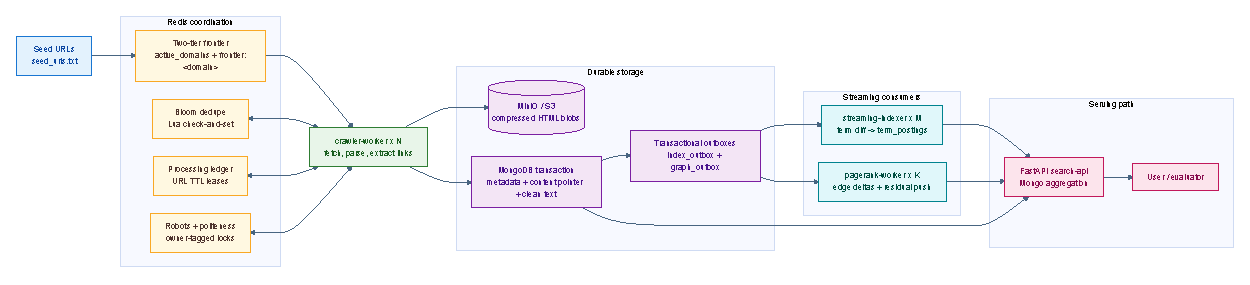
\includegraphics[width=\textwidth,height=0.78\textheight,keepaspectratio]{figures/architecture.pdf}

  \vspace{0.3em}
  \small Full architecture: Redis coordination, crawler workers, MinIO blob storage, MongoDB records, streaming consumers, and search API.
\end{frame}

\begin{frame}{Docker Compose Topology}
  \begin{columns}[T,totalwidth=\textwidth]
    \begin{column}{0.50\textwidth}
      \component{Docker Compose}
      {Runs Redis, MongoDB, MinIO, crawler workers, streaming indexer, PageRank worker, search API, and seed helper as containers.}
      {It gives a reproducible setup where every service runs in an isolated container with the same network and environment.}
    \end{column}
    \begin{column}{0.46\textwidth}
      \begin{block}{What Docker gives us}
        \begin{itemize}
          \item Same setup for every evaluator machine.
          \item Easy service startup and shutdown.
          \item Multiple crawler workers can run side by side.
          \item Services communicate using Compose DNS names.
        \end{itemize}
      \end{block}
    \end{column}
  \end{columns}
\end{frame}

\begin{frame}{Seed Helper}
  \component{Seed helper}
  {Reads \texttt{seed\_urls.txt} and inserts starting URLs into the Redis frontier.}
  {The crawler is pull-based. Workers need an initial frontier before they can start discovering more links.}

  \begin{block}{Role in the flow}
    The seed helper only starts the crawl. After that, crawler workers discover new links from downloaded pages and add those URLs back into Redis.
  \end{block}
\end{frame}

\begin{frame}{Redis: Coordination Layer}
  \begin{columns}[T,totalwidth=\textwidth]
    \begin{column}{0.52\textwidth}
      \component{Redis}
      {Stores the URL frontier, Bloom-filter dedupe bits, URL processing leases, domain locks, and robots/crawl-delay cache.}
      {Redis gives low-latency atomic coordination between many worker containers.}
    \end{column}
    \begin{column}{0.44\textwidth}
      \begin{block}{Key Redis structures}
        \begin{itemize}
          \item \texttt{crawler:active\_domains}
          \item \texttt{crawler:frontier:<domain>}
          \item \texttt{crawler:bloom}
          \item \texttt{crawler:processing}
          \item \texttt{lock:<domain>}
        \end{itemize}
      \end{block}
    \end{column}
  \end{columns}
\end{frame}

\begin{frame}{Crawler Worker}
  \begin{columns}[T,totalwidth=\textwidth]
    \begin{column}{0.50\textwidth}
      \component{crawler-worker}
      {Pulls URLs from Redis, checks politeness, downloads HTML, extracts clean text and outbound links, and writes page data to storage.}
      {It is autonomous and stateless except for shared Redis/Mongo/MinIO state, so many workers can run at once.}
    \end{column}
    \begin{column}{0.46\textwidth}
      \begin{block}{Worker loop}
        \begin{enumerate}
          \item Dequeue URL from Redis.
          \item Acquire domain politeness lock.
          \item Fetch page.
          \item Parse title, text, links.
          \item Save transaction + outbox events.
          \item Release URL lease.
        \end{enumerate}
      \end{block}
    \end{column}
  \end{columns}
\end{frame}

\begin{frame}{Robots.txt And Politeness}
  \component{Robots and politeness}
  {Fetches \texttt{/robots.txt}, checks \texttt{can\_fetch}, caches robots content and crawl-delay in Redis, and enforces per-domain locks.}
  {Distributed crawlers must be polite. Multiple workers should not attack the same domain simultaneously.}

  \begin{block}{Policy}
    If a URL is disallowed, it is not added to the frontier. If robots data is missing or unavailable, the current crawler policy allows crawling by default.
  \end{block}
\end{frame}

\begin{frame}{MinIO / S3 Blob Storage}
  \component{MinIO}
  {Stores compressed raw HTML blobs in the shared \texttt{crawler-html} bucket. MongoDB stores only pointers and metadata.}
  {Large HTML blobs should not bloat MongoDB's working set. Shared object storage also works when workers and API run on different machines.}

  \begin{block}{Data split}
    MongoDB keeps searchable metadata and references. MinIO keeps the heavier original page payloads.
  \end{block}
\end{frame}

\begin{frame}{MongoDB Storage}
  \small
  \component{MongoDB}
  {Stores page metadata, clean text, content pointers, indexing state, graph edges, and PageRank scores.}
  {MongoDB gives durable structured storage and supports atomic updates across the crawler pipeline.}

  \begin{block}{Main collections}
    \begin{itemize}
      \item \texttt{pages\_metadata}
      \item \texttt{pages\_content}
      \item \texttt{pages\_documents}
      \item \texttt{index\_outbox}
      \item \texttt{graph\_outbox}
      \item \texttt{term\_postings}, \texttt{graph\_edges}, \texttt{pagerank\_nodes}
    \end{itemize}
  \end{block}
\end{frame}

\begin{frame}{Streaming Indexer}
  \component{streaming-indexer}
  {Consumes \texttt{index\_outbox}, loads clean text from \texttt{pages\_documents}, tokenizes/stems terms, computes term frequencies, and updates \texttt{term\_postings}.}
  {Indexing is moved out of crawler workers, so crawling stays fast and search state is updated asynchronously.}

  \begin{block}{Search index shape}
    \texttt{term\_postings} stores one document per \texttt{(term, url)}, avoiding giant embedded posting arrays for frequent terms.
  \end{block}
\end{frame}

\begin{frame}{Incremental PageRank Worker}
  \component{pagerank-worker}
  {Consumes \texttt{graph\_outbox}, compares new outbound links with historical \texttt{graph\_edges}, applies PageRank contribution deltas, and updates \texttt{pagerank\_nodes}.}
  {Authority scoring is expensive graph math; separating it from crawling keeps the crawler responsive.}

  \begin{block}{How authority changes}
    When a page links to another page, it passes part of its authority forward. If the link graph changes after a recrawl, only the affected contributions are updated.
  \end{block}
\end{frame}

\begin{frame}{Search API}
  \component{FastAPI search-api}
  {Receives a query, tokenizes it, aggregates matching \texttt{term\_postings}, joins \texttt{pagerank\_nodes}, computes final score, sorts and limits inside MongoDB.}
  {Search stays fast because it does not crawl, tokenize all documents, or recompute PageRank at query time.}

  \begin{block}{Ranking formula}
    \[
      \text{final score} = \text{term score} \times \text{authority score}
    \]
  \end{block}
\end{frame}

\begin{frame}{Index And Search Flow}
  \centering
  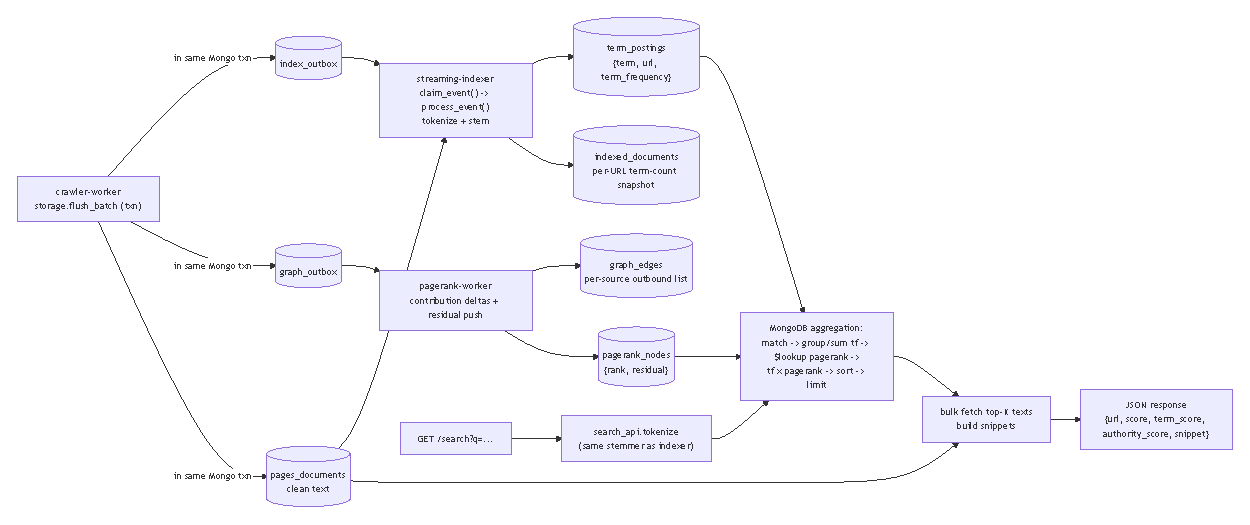
\includegraphics[width=0.92\textwidth,height=0.62\textheight,keepaspectratio]{figures/index_search_flow.pdf}

  \begin{block}{Result}
    Crawled text becomes searchable postings, PageRank becomes authority, and the API combines both signals when answering a query.
  \end{block}
\end{frame}

\begin{frame}{Fault Tolerance}
  \begin{columns}[T,totalwidth=\textwidth]
    \begin{column}{0.50\textwidth}
      \begin{block}{Failures handled}
        \begin{itemize}
          \item Worker dies mid-crawl.
          \item Duplicate URL discovery.
          \item Domain lock contention.
          \item Outbox consumer crash.
          \item PageRank transient write conflict.
        \end{itemize}
      \end{block}
    \end{column}
    \begin{column}{0.46\textwidth}
      \begin{block}{Mechanisms}
        \begin{itemize}
          \item Redis TTL leases.
          \item Lua atomic frontier updates.
          \item MongoDB transactions.
          \item Outbox claim/reclaim.
          \item PageRank recompute reset.
        \end{itemize}
      \end{block}
    \end{column}
  \end{columns}
\end{frame}

\begin{frame}{How One Page Moves Through The System}
  \begin{enumerate}
    \item A URL is selected from Redis according to priority and domain availability.
    \item A crawler worker checks robots.txt and waits for the domain lock if needed.
    \item The worker downloads HTML, extracts text, and discovers outbound links.
    \item Raw HTML is compressed into MinIO and page metadata is saved in MongoDB.
    \item Background workers update the search index and PageRank information.
    \item The Search API uses the prepared data to return ranked results quickly.
  \end{enumerate}
\end{frame}

\begin{frame}{Final System Summary}
  \centering
  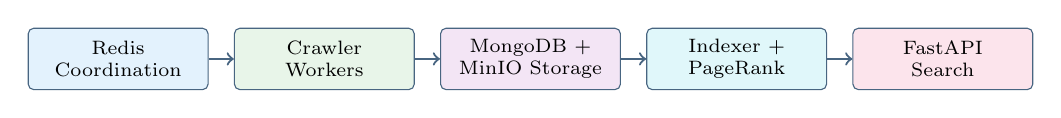
\begin{tikzpicture}[
      node distance=0.32cm,
      every node/.style={font=\scriptsize},
      box/.style={draw=Steel, rounded corners=2pt, minimum height=0.78cm, align=center, text width=2.05cm},
      arrow/.style={->, thick, draw=Steel}
    ]
    \node[box, fill=SoftBlue] (coord) {Redis\\Coordination};
    \node[box, fill=SoftGreen, right=of coord] (crawl) {Crawler\\Workers};
    \node[box, fill=SoftPurple, right=of crawl] (store) {MongoDB +\\MinIO Storage};
    \node[box, fill=SoftCyan, right=of store] (process) {Indexer +\\PageRank};
    \node[box, fill=SoftRose, right=of process] (serve) {FastAPI\\Search};

    \draw[arrow] (coord) -- (crawl);
    \draw[arrow] (crawl) -- (store);
    \draw[arrow] (store) -- (process);
    \draw[arrow] (process) -- (serve);
  \end{tikzpicture}

  \vspace{1.0em}
  \begin{block}{Main contribution}
    The project connects distributed crawling, polite URL scheduling, durable storage, streaming indexing, graph-based authority scoring, and ranked search into one Dockerized pipeline.
  \end{block}
\end{frame}

\end{document}
